\pagenumbering{gobble}

%****************************************
%*										*
%*										*
%****************************************
%HERE IS A GOOD COLLAGE OF PHOTOS, IT´S GOOD WITH PORTRAITS 
\begin{comment}

%BEGIN OF COLLAGE 
%BEGIN OF COLLAGE 
%BEGIN OF COLLAGE 
%BEGIN OF COLLAGE 
%BEGIN OF COLLAGE 

\newgeometry{margin=0cm}
\setlength{\parindent}{0pt}

\setlength{\tabcolsep}{0pt} 
\renewcommand{\arraystretch}{0}

\begin{tabular}{ l l l  }


\includegraphics[width=9.3cm,height=5.4cm]{./res/dummy.jpg} &

\includegraphics[width=9.3cm,height=5.4cm]{./res/dummy.jpg} & 

\includegraphics[width=9.4cm,height=5.4cm]{./res/dummy.jpg} \\


\includegraphics[width=9.3cm,height=5.4cm]{./res/dummy.jpg} &

\includegraphics[width=9.3cm,height=5.4cm]{./res/dummy.jpg} & 

\includegraphics[width=9.4cm,height=5.4cm]{./res/dummy.jpg} \\


\includegraphics[width=9.3cm,height=5.4cm]{./res/dummy.jpg} &

\includegraphics[width=9.3cm,height=5.4cm]{./res/dummy.jpg} & 

\includegraphics[width=9.4cm,height=5.4cm]{./res/dummy.jpg} \\


\includegraphics[width=9.3cm,height=5.4cm]{./res/dummy.jpg} &

\includegraphics[width=9.3cm,height=5.4cm]{./res/dummy.jpg} & 

\includegraphics[width=9.4cm,height=5.4cm]{./res/dummy.jpg} \\

\end{tabular}

\restoregeometry


%END OF COLLAGE 
%END OF COLLAGE 
%END OF COLLAGE 
%END OF COLLAGE 
\end{comment}

\begingroup
\thispagestyle{empty}
\AddToShipoutPicture*{\put(0,0){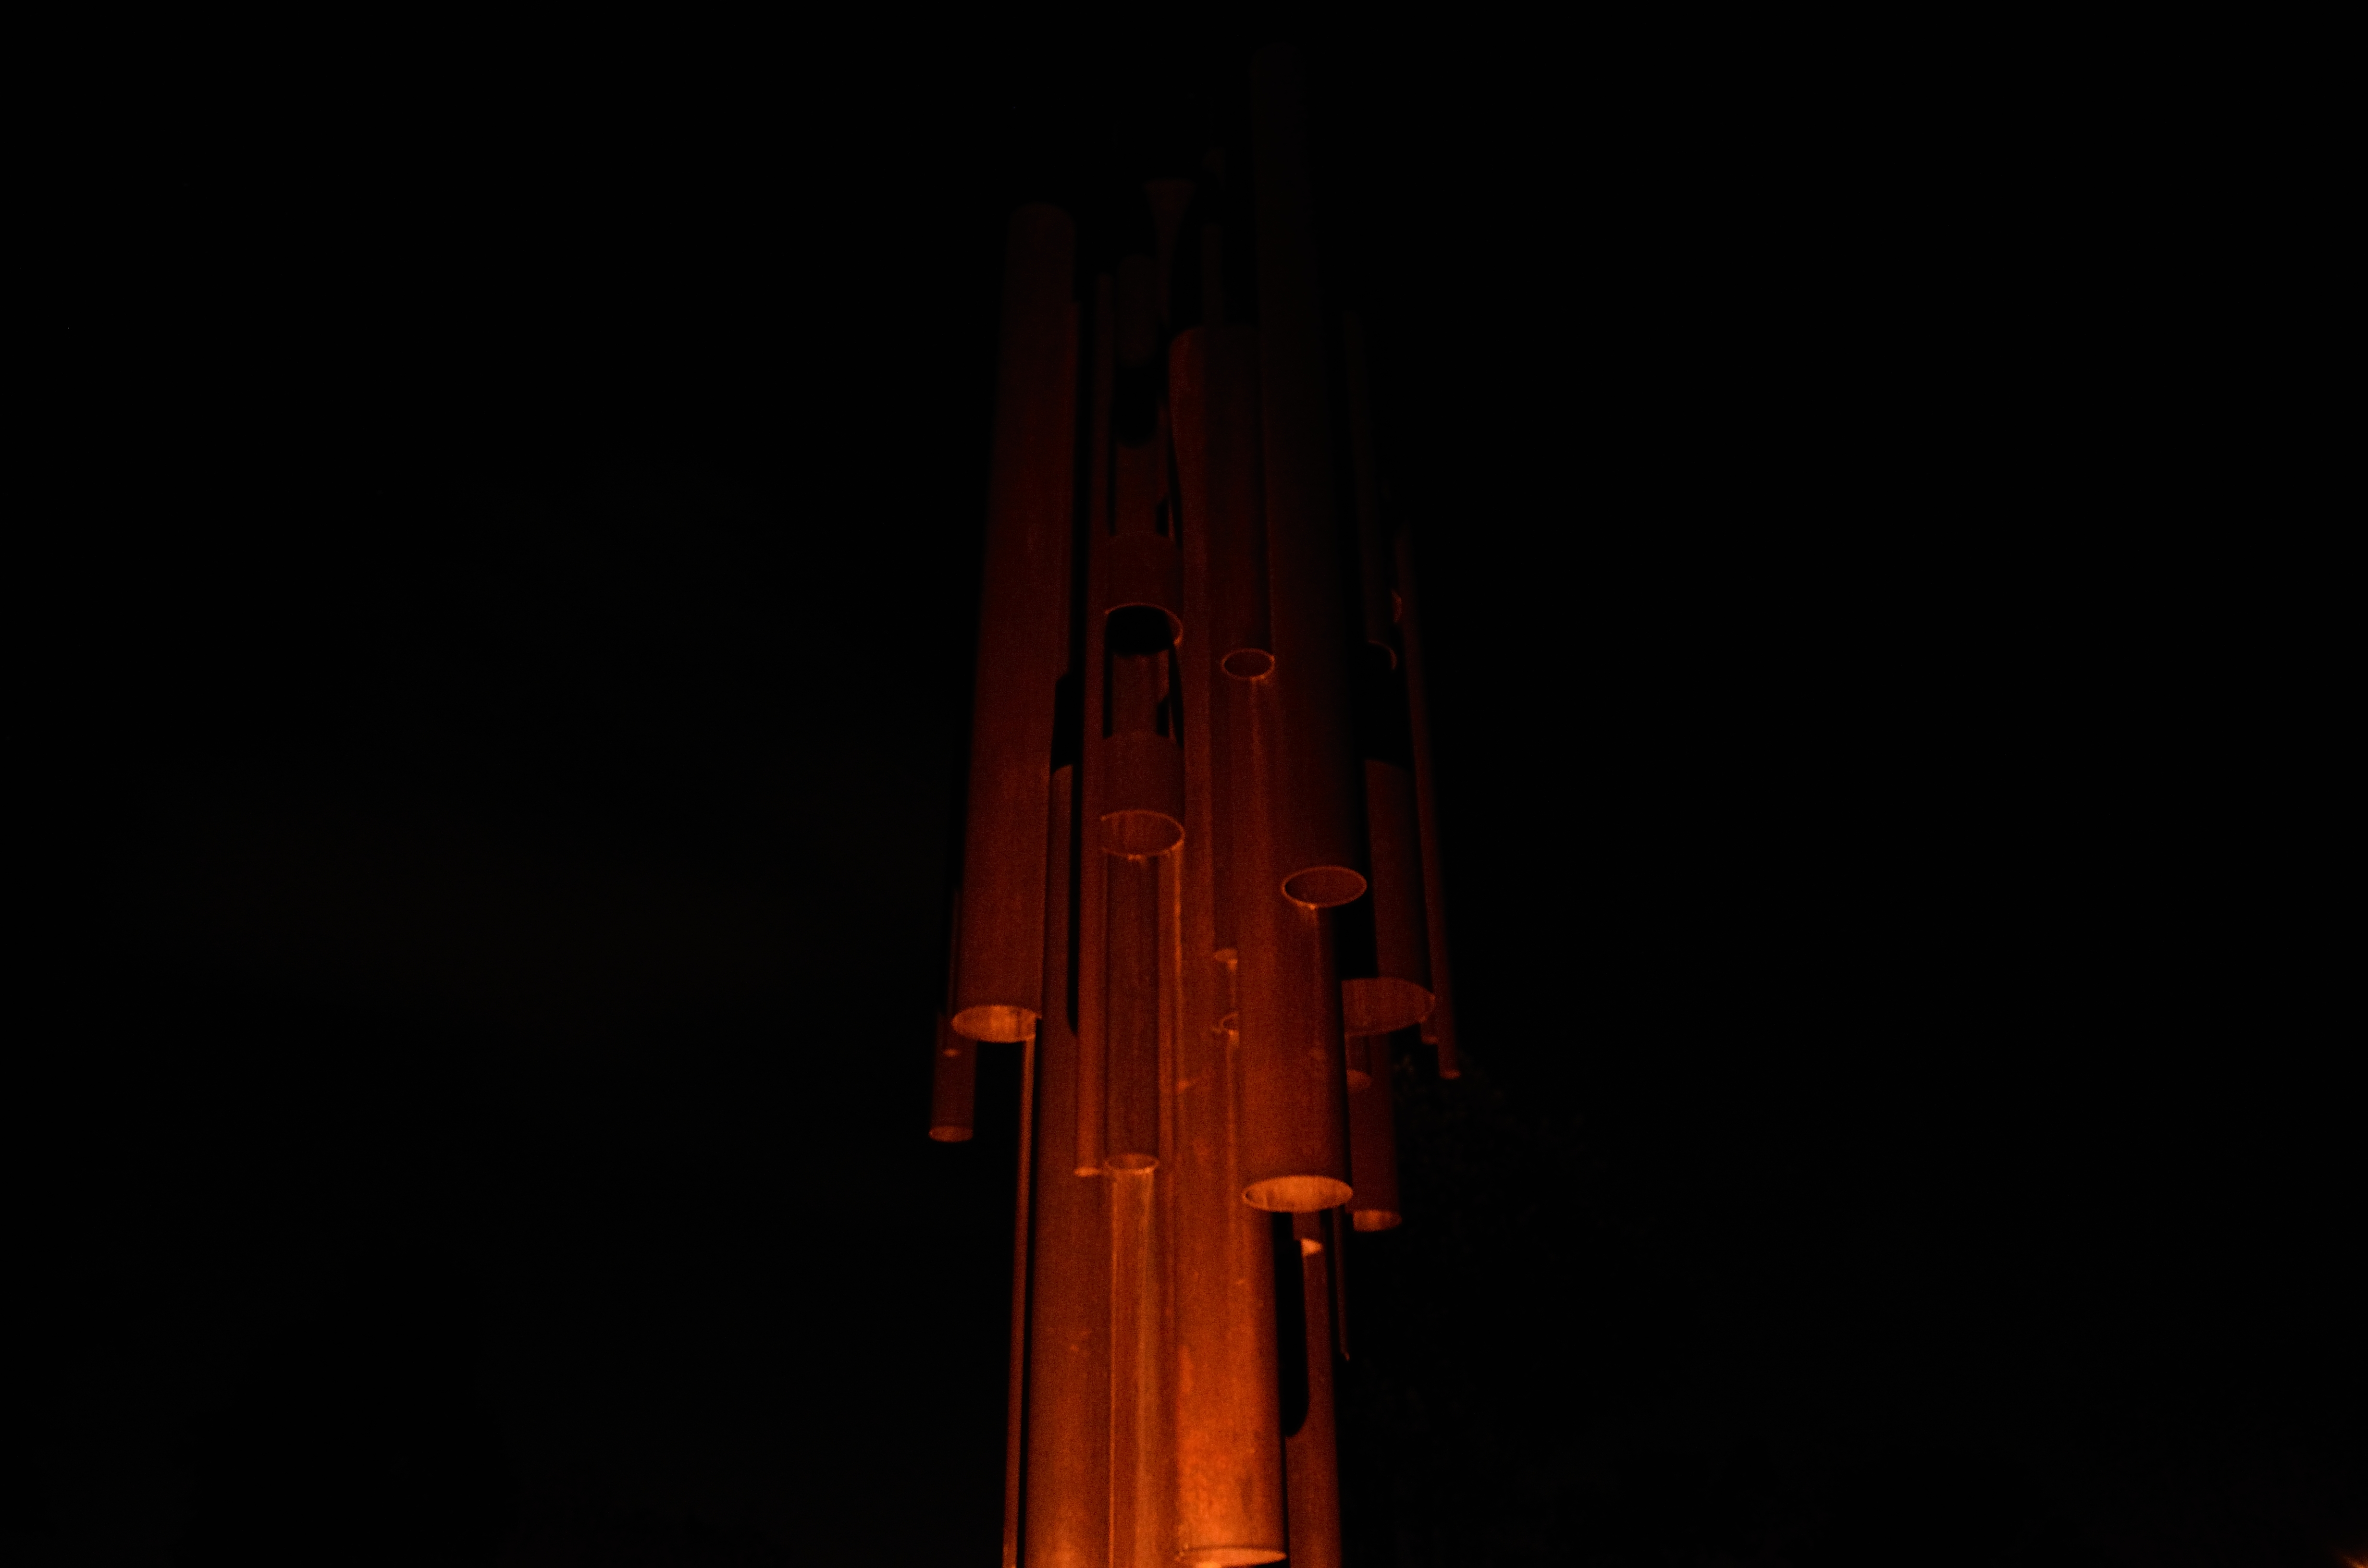
\includegraphics[scale=0.8]{./res/cover0.jpg}}} % Image background
\centering
\vspace*{5cm}
\endgroup

\newpage

%****************************************
%*										*
%*										*
%****************************************
\newpage
\newpage
\ClearShipoutPicture
\newpage

\vspace*{\fill}
\begin{center}
{\scshape\huge Landscape Book Template\par}
\vspace{1cm}
{\Large Ciro Iván García\par}
\end{center}
\vspace*{\fill}
\newpage

\newgeometry{left=3cm,right=3cm}
\setlength\columnsep{30pt} 
\begin{multicols}{2}

~\vfill

\noindent Template by: Ciro García \\
\noindent \textit{January 2018}

\columnbreak

\tableofcontents
\newpage

\end{multicols}

%****************************************
%*										*
%*				PAGE STYLE				*
%*										*
%****************************************
\pagenumbering{arabic}

%here its the code for the page number location and the header style 

\fancypagestyle{plain}{%
  \fancyhf{}
  \fancyfoot[EC]{%
      \begin{tikzpicture}[remember picture,overlay]
      %THIS PUT AN IMAGE AT THE ACTUAL SIDE
      	  %\node[xshift=2cm,yshift=1cm,font=\bfseries] (number) at (current page.west) {\includegraphics[height=24cm,width=4cm]{./res/side.png}};
          \node[circle,draw=black, line width=0.25mm,fill=white,xshift=2cm,yshift=-8cm,font=\bfseries] (number) at (current page.west) {\thepage};
      \end{tikzpicture}
  }%
  \fancyhead[ER]{\leftmark}
  
  \fancyfoot[OC]{%
      \begin{tikzpicture}[remember picture,overlay]
      	  %\node[xshift=-2cm,yshift=1cm,font=\bfseries] (number) at (current page.east) {\includegraphics[height=24cm,width=4cm]{./res/side.png}};
          \node[circle,draw=black, line width=0.25mm,fill=white,xshift=-2cm,yshift=-8cm,font=\bfseries] (number) at (current page.east) {\thepage};
      \end{tikzpicture}
  }%
  \renewcommand{\headrulewidth}{0pt}
}


\fancypagestyle{CustomFancy}{%
  \fancyhf{}
  \fancyfoot[EC]{%
      \begin{tikzpicture}[remember picture,overlay]
      	  %\node[xshift=2cm,yshift=1cm,font=\bfseries] (number) at (current page.west) {\includegraphics[height=24cm,width=4cm]{./res/side.png}};
          \node[circle,draw=black, line width=0.25mm,fill=white,xshift=2cm,yshift=-8cm,font=\bfseries] (number) at (current page.west) {\thepage};
      \end{tikzpicture}
  }%
  \fancyhead[EC]{\leftmark}
  
  \fancyfoot[OC]{%
      \begin{tikzpicture}[remember picture,overlay]
      	  %\node[xshift=-2cm,yshift=1cm,font=\bfseries] (number) at (current page.east) {\includegraphics[height=24cm,width=4cm]{./res/side.png}};
          \node[circle,draw=black, line width=0.25mm,fill=white,xshift=-2cm,yshift=-8cm,font=\bfseries] (number) at (current page.east) {\thepage};
      \end{tikzpicture}
  }%
  \fancyhead[OC]{\leftmark}
  \fancyheadoffset{-4cm}
}

\pagestyle{CustomFancy}




